\chapter{Pyridines}
Pyridines are described as six- membered heterocycles, which include a single N-atom in the ring. They are aromatic compounds and their  6 $\pi$-electrons are delocalized over the entire ring. All atoms in the ring are sp$^2$ hybridized. The N-atom has a lone pair which does not contribute to the aromatic system and has influence on the chemical properties of the pyridine.
It's hydrophilic and hydrophobic character makes it miscible with water and organic solvents. \cite{joule}

Pyridines can be involved in  protonation, alkylation, acylation and N-oxidation as  tertiary amines and nucleophilic substitution as aromatic compounds.

The compound itself is a weak ligand for forming complexes with transition metal ions, but its acid derivates can form strong complexes.

With a pk$_a$ of approximately 5 pyridines are weak bases and therefore the formation of salts is favored.
The electronegative nitrogen in the ring makes the pyridine an electron deficient molecule. Therefore it is more improbable for the compound to partake in electrophilic reactions unlike other benzene derivatives. Nucleophilic substitution and metalation, however, occur more often with pyridines and are conducted using strong organometallic bases. \cite{joule1}

\begin{figure}[htpb!]
\centering
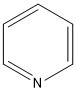
\includegraphics{figures/pyridine.jpg}
\caption{Chemical structure of pyridine}
\label{fig:py}
\end{figure}

\section{4-hydroxy-methyl-pyridine complexes}
\label{ch:4HOMP}
\renewcommand{\arraystretch}{1.3}
\begin{longtable}{|p{1\textwidth}|}

 \captionabove{List of in the CCDC published 4-hydroxy-methyl-pyridine complexes \cite{ccdc}}
 \label{tab:pubpy}\\
 \hline
 trans-[PtCl$_2$NH$_3$(4-(hydroxymethyl)-pyridine)] \cite{RamosLima20033379}\\
 \hline
 [Mn$_6$O$_2$(O$_2$CPh)$_10$(4-hydroxymethylpyridine)$_3$(MeCN)] \cite{Stamatatos20061737}\\
 \hline
 catena-(($\mu_2$-pyridine-2,6-dicarboxylato)-($\mu_2$-4-(hydroxymethyl)pyridine)-copper(II) \cite{Ucar2009}\\
 \hline
 Diaqua-(pyridine-2,6-dicarboxylato)-(4-hydroxymethyl)pyridine)-nickel(II) monohydrate \cite{Ucar2009}\\
 \hline
 [Ag(4-hydroxymethylpyridine)$_2$]NO$_3$ \cite{KalinowskaLis2014394}\\
 \hline
 trans-[PtCl$_2$(NH$_2$CH(CH$_3$)$_2$(4-py-MeOH))] \cite{KalinowskaLis20081328}\\
 \hline
 trans-[PtCl$_4$(NH$_3$)(4-py-MeOH)] \cite{KalinowskaLis20081328}\\
 \hline
 [Cu(4-pyridylmethanol)$_4$Cl]Cl \cite{monc2004}\\
 \hline
bis(Glycinato-N,O)-bis(4-hydroxymethylpyridine-N)-nickel \cite{zhao2010}\\
\hline
chloro-(2-(isobutylimino)methylphenolato)-((pyridin-4-yl)(methanol))-platinum dichloromethane solvate \cite{rahman2015}\\
\hline
bis(Niflumato-O)-bis(4-pyridylmethanol-N)-copper(II) methanol solvate \cite{maroszova2011}\\
\hline
Aqua-bis(2-chlorobenzoato-O)-bis(4-pyridylmethanol-N)-copper(II) \cite{maroszova2011}\\
\hline
tetrakis($\mu_2$-(2,6-Diisopropylphenyl)phosphato)-tetrakis(4-(hydroxymethylpyridine)-tetra-zinc \cite{murugavel2006}\\
\hline
bis($\mu_4$-Oxo)-tetrakis($\mu_3$-benzoato)-hexakis($\mu_2$-benzoato)-(acetonitrile)-tris(4-hydroxymethylpyridine)-tetra-manganese(II)-di-manganese(III) acetonitrile solvate \cite{stamatatos2006}\\
\hline
tetrakis($\mu_2$-acetato)-bis(4-pyridinemethanol)-di-rhodium)  \cite{ye2011}\\
\hline
(Cyclobutane-1,1-dicarboxylato)-(bis((pyridine-4-yl)methanol)-platinum \cite{escribano2013}\\
\hline
bis($\mu_2$-cyclohexane-1,2-dicarboxylic acid)-(tetrakis((pyridin-4-yl)methanol)-di-platinum dihydrate \cite{escribano2013}\\
\hline
catena-[tris($\mu_2$-Azido-N$^1$,N$^1$)-($\mu_2$-Azido-N$^1$,N$^3$)-tetrakis(4-hydroxymethylpyridine)-di-cadmium(II)] \cite{goher2008}\\
\hline
bis((pyridin-4-yl)methanol)-(trifluormethanesulfonato)-silver \cite{deBoer2014}\\
\hline
bis(pyridin-4-yl)methanol)-silver perchlorate \cite{deBoer2014}\\
\hline
bis((pyridin-4-yl)methanol)-silver tetrafluoroborate acetonitrile solvate \cite{deBoer2014}\\
\hline
tetrakis((pyridin-4-yl)methanol)-bis(thiocyanato)-nickel \cite{werner2015}\\
\hline
bis(ethanol)-bis((pyridin-4-yl)methanol)-bis(thiocyanato)-nickel \cite{werner2015}\\
\hline
diaqua-bis((pyridin-4-yl)methanol)-bis(thiocyanato)-nickel \cite{werner2015}\\
\hline
catena-[($\mu$-pyridin-4-ylmethanol)-($\mu$-thiocyanato)-(pyridin-4-ylmethanol)-(isothiocyanato-nickel] \cite{werner2015}\\
\hline
Aqua-bis(4-clofibriato-O)-bis(4-pyridylmethanol-N)-copper(II) dihydrate \cite{moncol2004}\\
\hline
tris(Tetraethylammonium)-tris($\mu_2$-4-pyridinemethanolato)-bis(tricarbonyl-tungsten(0)) acetonitrito solvate \cite{klausmeyer2004}\\
\hline
chloro-tetrakis(pyrid-4-ylmethanol-N)-copper(II) chloride \cite{moncol2004}\\
\hline
trans-dichloro-isopropylamine-(4-(hydroxymethyl)pyridine-N)-platinum(II) \cite{ramoslima2006}\\
\hline
bis(pyridin-4-yl-N)methanol)-silver nitrate \cite{deBoer2014}\\
\hline
catena-($\mu_2$-Pyridin-4-ylmethanol)-($\mu_2$-thiocyanato-N,S)-isothiocyanato-(4-(hydroxymethylpyridine)-cadmium) \cite{werneracta}\\
\hline
Tetrakis($\mu_2$-Acetato-O, O')-bis(4-pyridylmethanol-N)-di-copper(II) \cite{hoang1993}\\
\hline
Aqua-bis(-bromobenzoato-$\kappa$O)-bis(4-pyridylmethanol-$\kappa$N)-copper(II) \cite{moncol2008}\\
\hline
catena-[($\mu$-adipato)-bis((pyridin-4-yl)methanol)-aqua-copper] \cite{chechova2015}\\
\hline
\end{longtable}
 
 \section{4-methoxy-pyridine complexes}
 \label{ch:4MOP}
 \begin{longtable}{|p{1\textwidth}|}
 
 \captionabove{List of in the CCDC published 4-methoxy-pyridine complexes \cite{ccdc}}
 \label{tab:pubmepy}\\
 \hline
 bis(acetonitrite)-tetrakis(4-methoxypyridine)-di-silver dihexafluorophosphate \cite{wong2015}\\
\hline
 bis($\mu_2$-iodo)-bis(4-methoxypyridine)hexamethyl-di-platinum \cite{gosh2015}\\
 \hline
 diaqua-(chelidamato)-(4-methoxypyridine)-nickel(II) dihydrate \cite{ucar2015}\\
 \hline
 diaqua-(chelidamato)-(4-methoxypyridine)-cobalt(II) dihydrate \cite{ucar2015}\\
 \hline
 tetrakis(4-methoxypyridine)-dioxo-rhenium(V) hexafluorophosphate \cite{canlier2010}\\
 \hline
 (4-Methoxypyridine)-(pyridine-2,6-dicarboxylato-N,O,O')-copper(II) \cite{perry2004}\\
 \hline
 bis(cyano)-(tetrakis(4-methoxypyridine))-ruthenium \cite{pieslinger2013}\\
 \hline
bis($\mu_2$-cyano)-dichloro-octapyridyl-tetrakis(4-methoxypyridine)-tri-ruthenium bis(hexafluorophosphate) \cite{pieslinger2013}\\
\hline
chloro-(p-methoxypyridine)-(2-(2-pyridyl)phenyl)-platinum(II) chloroform \cite{godbert2007}\\
\hline 
(benzo(h)quinolin-10-yl)-chloro-(p-methoxypyridine)-platinum(II) \cite{godbert2007}\\
\hline
bis(acetato)-aqua-bis(4-methoxypyridine)-cadmium \cite{saxena2015}\\
\hline
catena-(bis-$\mu_4$-Benzene-1,3-dicarboxylato)-bis(4-methoxypyridine)-di-zinc(II) methanol  ciathrate \cite{abourahma2003}\\
\hline
catena-(bis$\mu_4$-Benzene-1,3-dicarboxylato)-bis(4-methoxypyridine)-di-zinc(II) benzene ciathrate) \cite{abourahma2003}\\
\hline
tricarbonyl-(4-methoxypyridine)-pyridine-2-carboxylato)-rhenium \cite{hayes2015}\\
\hline
cis-1,2-Dichlorovinyl(4-methoxypyridine)-cobaloxime chloroform solvate \cite{follet2007}\\
\hline
Tetracarbonyl-(4-methoxypyridine)-(triphenylphosphine)-tungsten \cite{carlton2013}\\
\hline
catena-($\mu_3$-1,2-Benzoisothiazole-3-thionato-1,1-dioxide-S,S,S)-($\mu_2$-1,2-benzoisothiazole-3-thionato-1,1-dioxide-S,S)-bis(4methoxypyridine)-di-silver(II) \cite{dennehy2010}\\
\hline
($\eta^2, \eta^2$-Cyclo-octa-1,5-diene)-(4-methoxypyridine)-tricyclohexylphosphine-iridium hexafluorophospate \cite{mantilli2012}\\
\hline
bis(4-methoxypyridine)(propane-1,3-diylbis(diphenylphosphine)-platinum bi(fluoromethanesulfonate) monohydrate \cite{weilandt2012}\\
\hline
bis(4-methoxypyridine)(propane-1,3-diylbis(diphenylphosphine)-palladium bis(fluoromethanesulfonate) monohydrate \cite{weilandt2012}\\
\hline
Chloro-(dihydrogen dimethyl glyoximato)-(4-methoxypyridine)-(dimethyl glyoximato)-cobalt diethyl ether solvate \cite{wakerley2014}\\
\hline
bis(4-methoxypyridine)-(2,2'.6',2''.6'',2'''-quaterpyridine)-ruthenium diperchlorate monohydrate \cite{liu2014}\\
\hline
(3,5-di-t-butylcatexholato)-(3,5-di-t-butyl-o-semiquinonanto)-bis-(4methoxypyridine)-cobalt(II) \cite{schmidt2010}\\
\hline

 \end{longtable} 
 
 
 \section{Comparison between 4-HOMepy and 4-MeOpy}
 4-Hydroxymethylpyridine (4-HOMP) is an alcohol. By removing the H-atom of the alcohol group, metal atoms can bind to the oxygen of the formed alkoxid group. Due to this, 4-HOMP can be used as a bridging ligand. \\
However, this is not possible for 4-methoxypyridine (4-MOP). Hydrogen abstraction from its ether moiety is too unlikely. Thus, it can not from an additional bond, rendering 4-MOP unable to be used as a bridging ligand.\\
With a melting point of 52-56$^\circ$C and a boiling point of 107-110$^\circ$C 4-HOMP is a solid at room temperature and should be stored in the fridge. 4-Methoxypyridine has the same boiling point but a melting point at 4$^\circ$C and is therefore a liquid at 20$^\circ$C. \cite{sigma} \cite{sigma2}
